\MakeLinkTarget*{retypeset-note}
\pdfbookmark{ReTypeset Note}{retypeset-note}
\chapter*{\centerline{ReTypeset Note}}
\begingroup 
\normalsize
% 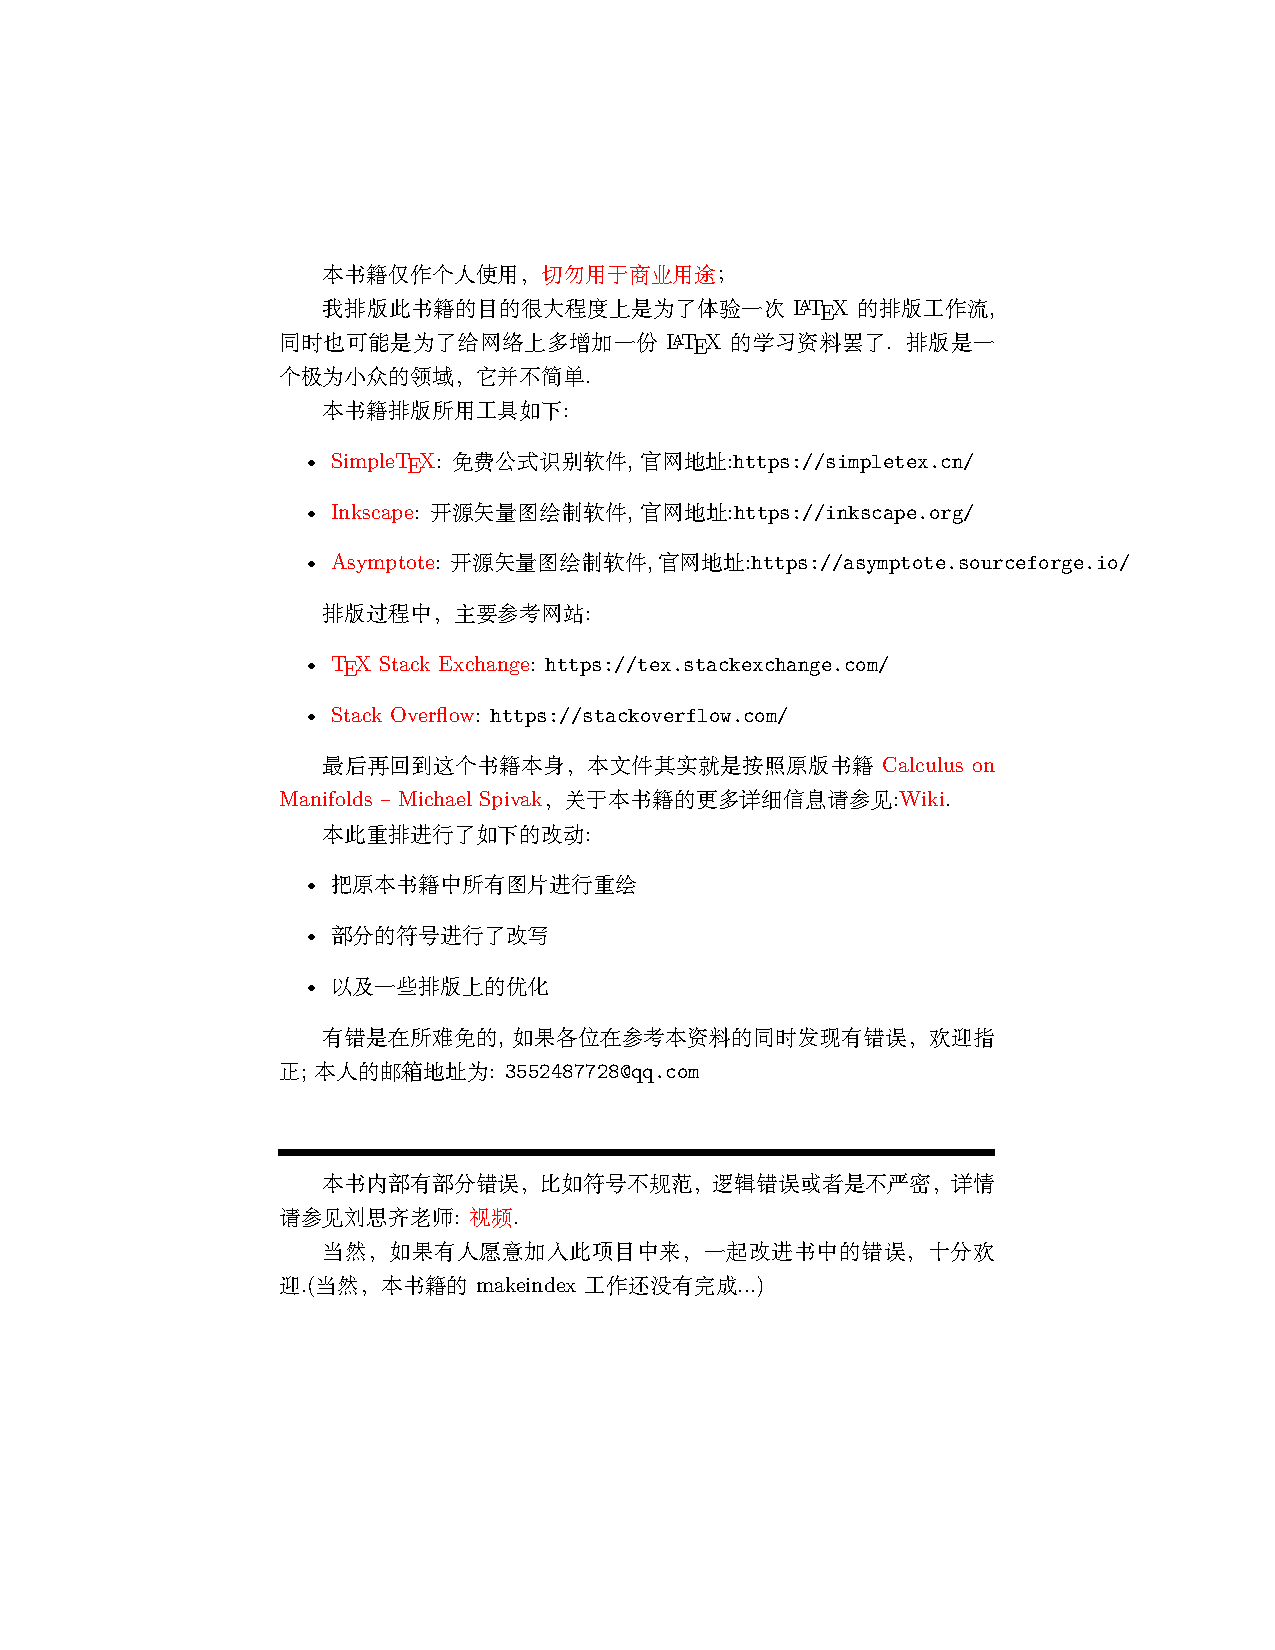
\includepdf{./chapter/NoteThat.pdf}
\newcommand{\red}[1]{{\sffamily #1}}
\thispagestyle{empty}
\noindent\framebox[\textwidth]{
  This book is for personal use only; \red{Commercial use is strictly prohibited}.
}
\vskip2.5em
The primary purpose of typesetting this book was to explore the \LaTeX{} typesetting workflow. 
It may also serve as an additional learning resource for \LaTeX{} available online.

The tools used in typesetting this book include: 
\begin{itemize} 
  \item \red{Simple\TeX{}}: \texttt{https://simpletex.cn/} 
  \item \red{Inkscape}: \texttt{https://inkscape.org/} 
  \item \red{Asymptote}: \texttt{https://asymptote.sourceforge.io/} 
\end{itemize}

Main websites referenced during the typesetting process: 
\begin{itemize} 
  \item \red{\TeX{} Stack Exchange}: \texttt{https://tex.stackexchange.com/} 
  \item \red{Stack Overflow}: \texttt{https://stackoverflow.com/} 
\end{itemize}

Back to the book itself—this document is a re-typeset version based on the original 
book \red{Calculus on Manifolds by Michael Spivak}. For more details about the book, 
see the Wikipedia page: \href{https://en.wikipedia.org/wiki/Calculus\_on\_Manifolds\_(book)}{Calculus\_on\_Manifolds -- Wiki}.

The re-typeset version includes the following changes: \begin{itemize} \item All original figures have 
been redrawn \item Some symbols have been modified \item Various typesetting improvements \end{itemize}

Mistakes are inevitable. If you notice any errors while referencing this material, feel free to point them out.
My email address is: \texttt{3552487728@qq.co}m

There are some errors in this book, such as inconsistent notation, logical flaws, or lack of rigor.
You can refer to Professor Siqi Liu's video: \texttt{https://b23.tv/bMRtbA6}.

\begin{leftbar}
  \noindent Typesetting is a highly niche field -- and it's far from simple.

  Of course, if anyone is interested in joining this project to help improve the book, 
  feel free to PR this Repo.
\end{leftbar}
\endgroup